\documentclass[11pt]{beamer}
% \usepackage[UTF8,space,hyperref]{ctex}
% \usepackage{listings}
% \usetheme{warsaw}
\usepackage{graphicx}
\author{Jie Ma}
\title{Reinforement Learning in Portfolio Management}

\begin{document}
\frame{\titlepage}

\begin{frame}[c]\frametitle{Introduction}
    Prices:
    \begin{align*}
        S^{k}=(S_{1}^{k},\cdots,S_{L}^{k})
    \end{align*}
    Portfolio:
    \begin{align*}
        P^{k}=(P_{0}^{k},P_{1}^{k},\cdots,P_{L}^{k})
    \end{align*}
    States:
    \begin{align*}
        State^{k}=(S^{k-N},S^{k-N+1},\cdots,S^{k-1},S^{k},P^{k-1})
    \end{align*}
    Rewards
    \begin{align*}
        R^{k}=R_{P^{k}*S^{k+1}-P^{k}*S^{k}}-switch\_cost
    \end{align*}
\end{frame}

\begin{frame}[c]\frametitle{Improvement}
    \begin{enumerate}
        \item State: add major indexes, add cash/riskless asset into portfolio
        \item Rewards: Improve Reward function from return to return/risk
        \item Frequency: Improve the price frequency means improving the sensitivity of agent
    \end{enumerate}
\end{frame}

\begin{frame}[c]\frametitle{works}
    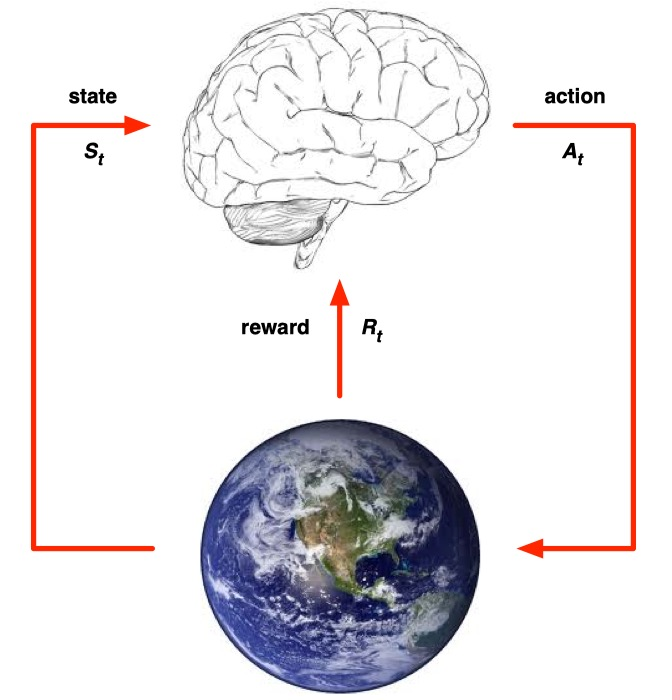
\includegraphics[scale=0.2]{rl_intro.jpg}
    \begin{itemize}

    \item Interpretation:
    \begin{itemize}

        \item Interpretation:
        \end{itemize}
    \item yes sir
    \end{itemize}
\end{frame}

\begin{frame}[c]\frametitle{Build Environment: Backtest System}
    \begin{block}{Logic of backtest system}
    initialize()\\
    while t in time.index:\\ \ \ \ \ pre\_trading()\\ \ \ \ \ strategy\_sigal()\\ \ \ \ \  strategy\_order()\\ \ \ \ \ after\_trading()
    \end{block}
\end{frame}

\begin{frame}[c]\frametitle{works}
Github:
\begin{align*}
    https://github.com/marsMa/rl\_in\_portfolio\_management
\end{align*}

\end{frame}

\end{document}